\documentclass[twoside,11pt]{article}
\showboxdepth3
\showboxbreadth10
\tracingonline1
% Any additional packages needed should be included after jmlr2e.
% Note that jmlr2e.sty includes epsfig, amssymb, natbib and graphicx,
% and defines many common macros, such as 'proof' and 'example'.
%
% It also sets the bibliographystyle to plainnat; for more information on
% natbib citation styles, see the natbib documentation, a copy of which
% is archived at http://www.jmlr.org/format/natbib.pdf

\usepackage{jmlr2e}
\usepackage{hyperref}
%\usepackage{parskip}

% Definitions of handy macros can go here
\newcommand{\dataset}{{\cal D}}
\newcommand{\fracpartial}[2]{\frac{\partial #1}{\partial  #2}}
% Heading arguments are {volume}{year}{pages}{submitted}{published}{author-full-names}

% Short headings should be running head and authors last names
\ShortHeadings{95-845: AAMLP Article}{Redd and Roberts}
\firstpageno{1}

\begin{document}

\title{Heinz 95-845: Predicting Futures Data\\ using Weather Data:\\ A Neural Network Approach}

\author{\name Andrew Redd \email aredd/aredd@andrew.cmu.edu \\
       \addr Heinz College\\
       Carnegie Mellon University\\
       Pittsburgh, PA, United States
       \AND
       \name Alexander Roberts \email adr1/adr1@andrew.cmu.edu \\
       \addr Heinz College\\
       Carnegie Mellon University\\
       Pittsburgh, PA, United States}


\maketitle

\begin{abstract}
  The futures market is used worldwide to hedge against price changes in commodities. Successful prediction of the future value of a good opens an abitrage opportunity on that future price. This paper discusses methods to predict the future value of one such commodity, Hard Red Wheat (HRW) using Recurrent Neural Networks (RNNs). Soft Red Wheat is grown primarily in Nebraska, Oklahoma, and Kansas. Our methods incorporate Automated Surface Observing Systems (ASOS) weather readings provided by the National Oceanic and Atmosphereic Administration (NOAA) in an effort to improve prediction outcomes.
\end{abstract}

\section{Introduction}

Although many factors influence the future price of HRW wheat in the US, we claim that the main drivers in predicting future wheat price are historic movement in the future, and weather. The purpose of this paper is to highlight several neural network models that use historic financial data and NOAA ASOS weather readings to predict the price of a wheat future 30 days into the future. The majority of literature on modeling financial markets is proprietary. Of the available literature, many of attempted to use historic futures contract price movement to predict future movement, but our research has not found a single instance of incorporating weather data to improve the model prediction. 

\subsection{Futures Contracts}
The future is risky. Individuals have a heterogeneous perception of future outcomes. This heterogeneity of belief combined with the heterogeneity of risk aversion among individuals creates risk gaps that can be filled by contractually. These contracts reduce risk by specifying how both parties will act in the future in regards to supplying and demanding goods. Producers, consumers and investors globally are able to speculate on perceived outcomes by contracting to buy or sell an item in the future at a locked-in price. The value of the option to buy at this locked-in price is therefore the market's consensus of the future price of a good given all current information. A model that could more effectively translate current information into the realized future price would aid in arbitraging the difference between the current and future price.

\subsection{The US Wheat Market}
Wheat is the third most-planted crop in the US. It first began trading on the futures market in 1877. Hard Red Winter Wheat is an important component of the US wheat market, being integral for most baking needs throughout the US. HRW wheat is primarily grown a relatively small geographic area across Oklahoma, Kansas and Nebraska. (\cite{CME}) As a result HRW wheat's risk profile is relatively less diversified when compared to other commodities. This geographically tight growing area makes HRW a good target for weather-based futures prediction. 

\subsection{Paper Structure}
In Section \ref{background}, we define key topics in futures trading. In Section \ref{model}, we provide a high-level overview of Recurrent Neural Nets (RNNs) and RNN layers such as Long-Short Term Memory (LSTM) and Gated Recurrent Units (GRU). Section \ref{experiment} describes the data sources and data preparation that lead up to the RNN model.  In Section \ref{results}, we discuss the efficiency of our predictions in terms of MSE. 

\section{Background} \label{background}

\subsection{Futures Trading}
	A futures contract is defined as "an agreement to buy or sell an underlying financial instrument or commodity at a specified future date and price." Why would this instrument be important in the economy? This contract enables producers to hedge risk and speculators to take on risk in relation to a given commodity. (\cite{InvestopediaF})
	
  Producers that would be interested in hedging risk through futures are players at any stage of product that depends on a commodity as an input. Imagine a wheat farmer, who in anticipation of a bumper year across the Midwest, desires to lock in today's high futures price rather than waiting three months to harvest and sell at the possibly low market price. Further imagine a bread manufacturer, who fears international wheat demand may cause a spike in price in the US wheat market, wishes to lock-in the current low futures price to better manage company's operations and pricing. In both cases, the producers feared a price change and used a futures contract to hedge away risk.
  
  Speculators in the market are organizations that vary in opinion of how current events will influence the current projected price of a given commodity. An investor that purchases a futures contract anticipates that the fluctuate either up or down from the current price.

  Insert Long and Short position images side by side

  An investor in futures (speculator or producer) is defined to have entered a "long" position if he/she agrees to purchase a good at a specified time and price in the future. An investor is termed to have entered a "short" position if he/she agrees to deliver a good at a specified time and price in the future. If an investor enters a long futures position and the market price goes up \textdollar1 during any daily time period, the investor has the option to purchase a more expensive good at a lower price in the future and thus profits \textdollar 1 per unit covered by the contract. Conversely, if the price of the good drops, the investor loses \textdollar 1 per unit covered by the contract. The opposite case holds true for the short position and market changes held constant.
  
  Futures contracts have two types of settlements. The first type is a cash settlement. This setting involves paying the cash difference between the futures contract price and the spot/market price at the time of contract expiration. The second type is physical delivery which requires the provider of the contract to deliver the actual goods. This applies to commodities such as oil, energy, and farm animals. The majority of futures contracts are settled via a cash settlement.
  
  Investors often wish to maintain a position (long/short) in a given commodity for a longer period of time than the specified contract duration. In this case the contract is rolled over "by closing the initial contract and opening a new longer-term contract for the same underlying asset at the then-current market price." \cite{InvestopediaRF}

  While many other strategies exist in futures trading, the defined long and short positions provide sufficent context for the motivation behind a better mechanism to predict the futures price.
 
\subsection{Weather's Impact on Wheat}
	
	Wheat quality has many measures such as protein content, grain structure, and grain weight. These quality measures are affected by a variety of variables such as soil quality, grain type, agronomy interventions, and growing climate conditions. Many studies have tried to model these effects in an effort to predict wheat yield within a time horizon to improve yield through intervention. \cite{Gooding2017} found that 70\% of crop variation could be accounted for by wheat type, fertilizer application, and precipitation during the winter and spring. Their model could account 90\% of the annual variation after including summer temperature. Further studies have shown that daily fluctuation measurements are critical to properly predicting wheat outcomes (\cite{Nuttall2017} \cite{Mearns1996})
	
\section{Method: Neural Networks} \label{model}

Since their development in the late 1980s, neural networks have become a mainstay in machine learning. (\cite{Schmidhuber2015}) Recurrent neural networks were designed to handle sequential information through a looping network structure that would pass data inputs to adjacent nodes. 

Insert RNN diagram here

Long-Short term memory (LSTM) and Gated Recurrent Units have been developed to further develop the idea of persistence of sequential effect. (\cite{Hochreiter1997}, \cite{Chung}) These methods provide even greater "memory" to the model, enabling networks to better work off of historic data. 

Insert side-by-side images of LSTM and GRU

[Insert more discussion on LSTMs and GRU]

These methods have been used in a myriad of sectors to provide a better prediction where other statistical methods have failed. (\cite{Ugurlu2018}) They have also proven useful in the prediction of stock patterns. (\cite{YoungohcYoon}) 

We use the keras to implement a series of models that use Simple RNN, LSTM, and GRU layers. \cite{chollet2015keras}. The implementation code can be found at \url{https://github.com/aredd-cmu/aa-project}


Guidance:
If you are combining existing methods, then you don't need to provide a ton of detail: feel free to just cite other packages and papers and tell us how you put them together.

\section{Methods} \label{Methods}

\subsection{Wheat Price Modeling Assumptions}
We assume that all non observed factors (fertilizer, soil quality, etc) are on average consistent throughout the wheat growing region. This assumption isolates weather as the primary indicator of crop yield and therefore wheat supply. We also assume that future demand is appropriately modeled by the futures price today. The final assumption is that predicted wheat supply is not accounting for all weather-related effects on the wheat crop and therefore wheat supply. These three assumptions isolate the current futures price and the weather as two main drivers of the true future price. 

%\emph{Note: if the paper is more about the application than the method, this Section may be entitled Methods and appear before Section \ref{model}}
%
%By reading the Experimental Setup, your reader should have the information necessary to replicate the study.
%
%Describe the cohort/data. Provide information about the population, the inclusion and exclusion criteria, what data were extracted, how features were processed, etc. In fact, you may want the following headings. \textbf{A flow chart can be very helpful} to illustrate the experimental setup, study design, inclusion/exclusion process, etc.
%
%For more clinical application papers, each of the sections above might be several paragraphs or pages because we really want to understand the setting
%\subsection{Cohort Selection} COMMENTED BECAUSE I DONT THINK WE NEED THIS
%Describe how the samples you used were selected to form your cohort and also to provide cohort descriptive statistics. In methodologic papers, the ``Table 1'' describing the population by covariate summary statistics goes here. In application papers, ``Table 1'' leads the Results Section. Relevant information about the study design, such how cases and controls were identified, goes here. See Section \ref{results} for an example of how to build a table in LaTeX.

\subsection{Data Extraction}

\subsection{Weather Data}
	The Automated Surface Observing System (ASOS) was commissioned in the early 90s with the intent of modernizing weather reporting in the US. For this project we used an API provided by Iowa State University that outputs daily aggregates of the minute data provided by ASOS. The output variables are listed in Appendix A: Weather Variable List.
	
	\subsubsection{Time Period Selection}
	The API calls retrieve weather data for a given time period at a given airport. We used a secondary called to identify all eligible airports in the Kansas, Oklahoma, and Nebraska. Even though ASOS was commissioned in the 90s much of the infrastructure was not in place until the early 2000s. We wanted to explore the trade off between more collection sites and a greater weather history. We determined the optimal time period by evaluating the number of operational stations in the ASOS system by year. We did this by pulling the data for every site across all three states for the years from 1998 - 2018 and received the output in Figure \ref{fig:asosstations}. 
	
	We defined an online station as having the number of rows that corresponded to one of the top three row numbers for the year. This method assumes that the majority of stations are operational with a full dataset and will thus define a "online" data size in number of rows by multiple votes. The year period that we chose was 2005 to 2018.
	
	\textit{NOTE: The anomaly from 2007-2009 seems to be an API issue related to those specific years. We still get data for those years in 2004-2005 periods.}
	
	\begin{figure}[htbp]
		\centering
		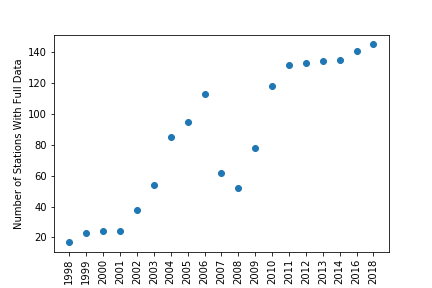
\includegraphics[width=3in]{ASOSstations.png}
		\caption{ASOS Online Stations over Time}
		\label{fig:asosstations}
	\end{figure}

	One concern related to choosing the appropriate time period relative to the number of online stations was that of losing our representative weather spread across the geographic region. We verified that our 2005 decision didn't remove more rural stations from the data set by visualizing a map of values across the geographic region shown below in Figure 
	
	\begin{figure}[htbp]
		\centering
		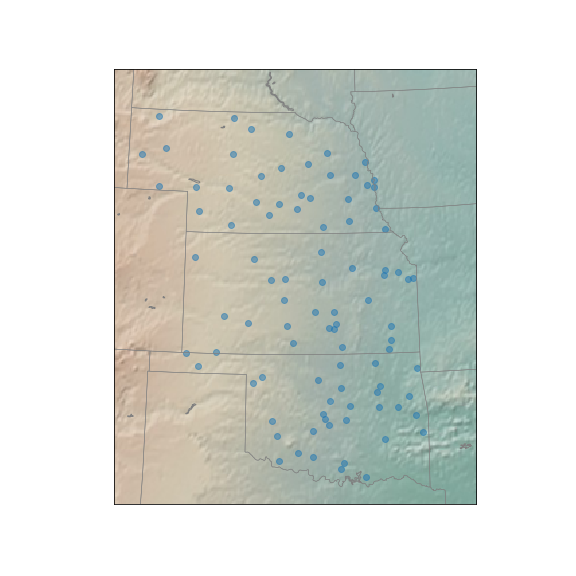
\includegraphics[width=3in]{ASOSspread.png}
		\caption{ASOS Online Stations over Time}
		\label{fig:asosspread}
	\end{figure}
	
	\subsubsection{Cleaning Data}
	First, The aggregated data had severe outliers along multiple columns due likely to sensor malfunction. (i.e. Max temperature of 921,613$^oF$) We handled these outliers using the following heuristics found via weather extremes recorded online shown in Table \ref{tab:bounds}. Since the values were large, conventional outlier methods weren't getting the variable ranges down to expected even after method application.  

	\begin{table}[htbp]
		\centering
		\begin{tabular}{lclc}
			Variable & Upper Bound & Lower Bound(\%) \\
			\hline \\[-11pt]
			max\_temp\_f & 130 & min(-50, min(min\_temp\_f))\\
			min\_temp\_f & 130 & -50 \\
			max\_dewpoint\_f & 90 & -20\\
			min\_dewpoint\_f & 90 & -20\\
			precip\_in & 70 & 0\\
			\hline
		\end{tabular}
		\label{tab:bounds}
		\caption{List of upper and lower bounds used to clean data outlier observations due to sensor malfunction}
	\end{table}

	Second, several of the values across the dataset were missing. Assuming that the data was lost because of a weather or geographically related sensor malfunction, we assert that the data is missing at random and impute based on our data values. The data was imputed assuming the variables followed a multivariate normal distribution using the Amelia II implementation in R. (\cite{ameila})
	
	Finally, the data was transformed into wide format in preparation for the merge with the futures data. 

\subsection{Futures Data}
 
We retrieved the futures prices directly from the Chicago Mercantile Exchange. The raw data form of the output was high, low, close, volumn and adjusted close. We decided to use the three month rollover strategy as a it would have less volatility in price due to contract changes (i.e. three months prior to contract termination, the current contract is sold and the next contract period is purchased)

The data output was relatively clean coming out of the CME API. We made minor changes to date and price format to work with our models. A full picture of our data pipeline is shown in figure \ref{fig:datapipeline}. We continue our discussion of the later end of the data pipeline with the results in section \ref{results}.

	\begin{figure}[htbp]
	\centering
	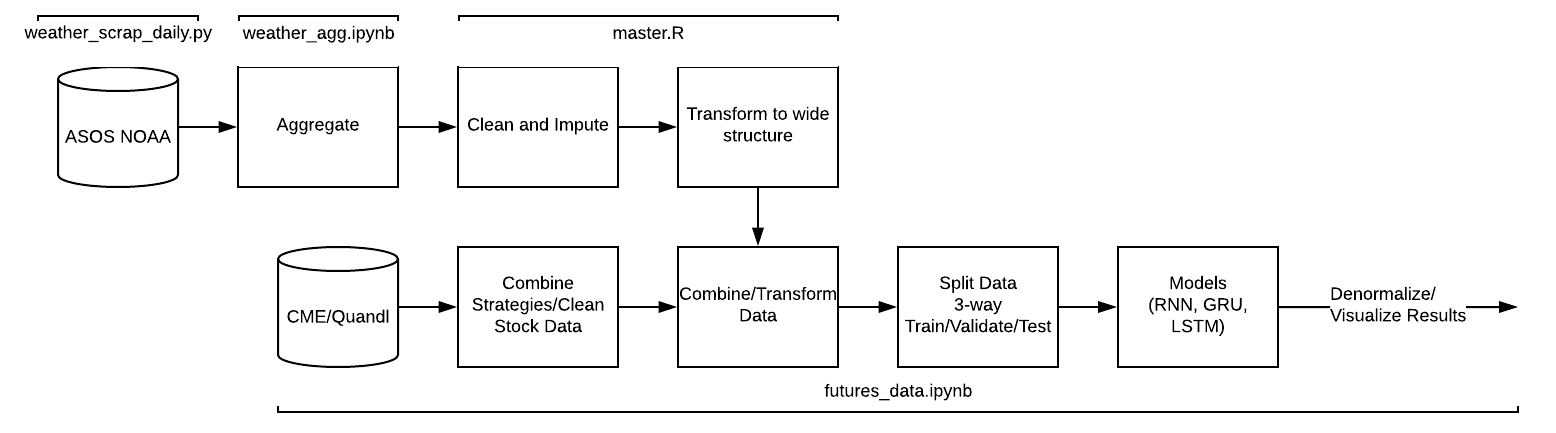
\includegraphics[width=5in]{DataPipeline.png}
	\caption{Data pipeline overview}
	\label{fig:datapipeline}
\end{figure}

\subsection{Feature Choices}

Many traders will use technical analysis in order to capture an ongoing trend in the financial product. We used Open-High-Low-Close (OHLC) average, daily percent change, and 50, 100, and 200 moving averages in order to communicate such trends.  

In this phase we also transformed our data into a sequence appropriate for an RNN. This sequence involved taking a sliding window along our dataset. The sliding window size we implemented was 44 working days (~ 2 mo.). We then crafted our target as a look-ahead variables 22 working days into the future. The output to this process is a matrix shaped (\# of windows (nrows - window size - look-ahead value), window size, ncols). The sequential nature of the input means that our inputs are no longer i.i.d., but as we are concerned with sequence of events this seems to be appropriate. In our baseline model (feed forward neural net) we do not perform this transformation and assume i.i.d. observations. 

\subsection{Comparison Methods}

In order to 

\begin{table}[htbp]
	\centering
	\begin{tabular}{lclc}
		Method & Outcome (\%) \\
		\hline \\[-11pt]
		Us & 20.1 \\
		Baseline & 18.2 \\ \hline
	\end{tabular}
	\label{tab:example}
	\caption{Outcome by method used. These are our results.}
\end{table}

To evaluate your model, often times you will compare against existing models.
If so, include them here with a brief description, citation, and any tweaks you made for your experiment.

Current Period Price - Profit will be zero because we will never speculate on price
difference

  Talk about mean loss/gain and variance in taht daily gain
  Talk about market volatility in the test period vs the train/validate period

\subsection{Evaluation Criteria}

RMSE


\begin{table}[htbp]
	\centering
	\begin{tabular}{lclc}
		Method & Outcome (\%) \\
		\hline \\[-11pt]
		Us & 20.1 \\
		Baseline & 18.2 \\ \hline
	\end{tabular}
	\label{tab:example}
	\caption{Outcome by method used. These are our results.}
\end{table}
  Show graph of profit as a function of day based on decisions. Current Price method will be a flat line at zero.
  On the current day, we purchase a futures contract and hold it until the 21 days passes and then sell the contract where all gains or losses are frozen on the transaction.
  Sum of the wins and losses, results in an overall loss or gain on the market.

explain why these are most useful measures of the outcome.

\section{Results} \label{results}

Compare the models' performance in terms of RMSE
Develop profit calculations here

Present the results here.
Do not describe how the results were obtained.
Those descriptions belong in Section \ref{experiment}.

Typically there are multiple parts and subparts of your study.
Use subsections to report the results.

\subsection{Results on Application A}

Give us some numbers about how well your method works, especially in comparison to some baselines.
You should provide a summary of the results in the text, as well as in tables (such as table~\ref{tab:example}) and figures (such as figure~\ref{fig:example}).

You may use subfigures/wrapfigures (LaTeX packages) so that figures don't have to span the whole page or multiple figures are side by side.

\begin{table}[htbp]
  \centering
  \begin{tabular}{lclc}
    Method & Outcome (\%) \\
    \hline \\[-11pt]
    Us & 20.1 \\
    Baseline & 18.2 \\ \hline
  \end{tabular}
  \label{tab:example}
    \caption{Outcome by method used. These are our results.}
\end{table}

\begin{figure}[htbp]
  \centering
  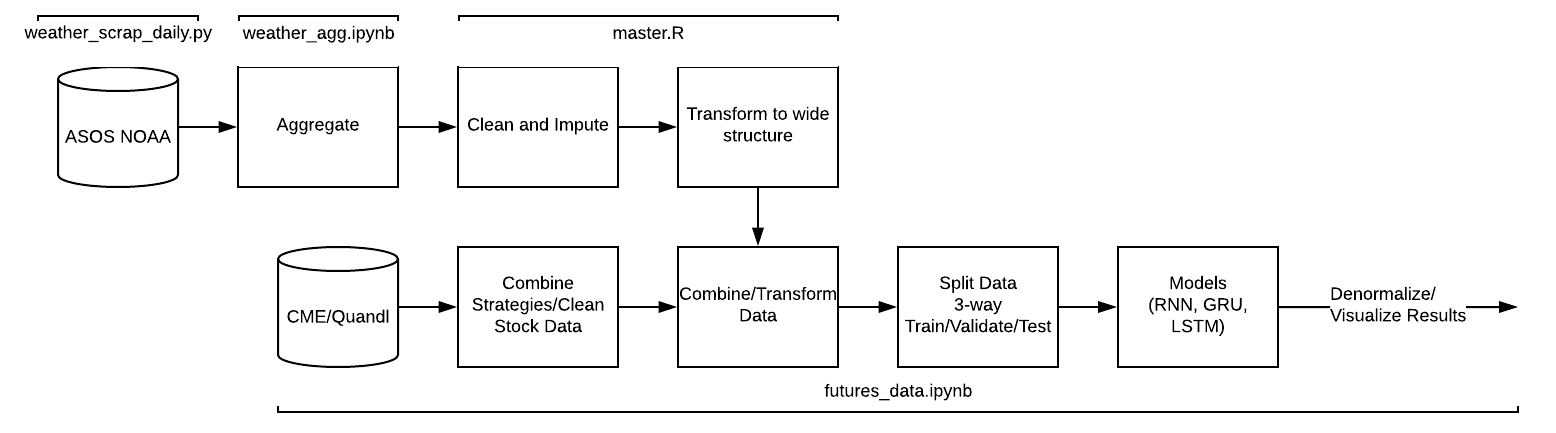
\includegraphics[height=4in]{DataPipeline.png}
  \caption{Example smile graphic.}
  \label{fig:example}
\end{figure}


% \begin{figure}
%         \begin{subfigure}[b]{0.25\textwidth}
%                 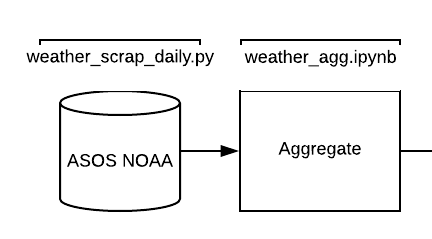
\includegraphics[width=\linewidth]{ASOSAgg.png}
%                 \caption{A gull}
%                 \label{fig:gull}
%         \end{subfigure}%
%         \begin{subfigure}[b]{0.25\textwidth}
%                 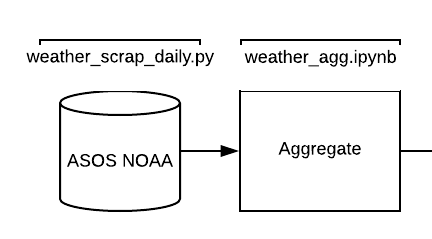
\includegraphics[width=\linewidth]{ASOSAgg.png}
%                 \caption{A gull2}
%                 \label{fig:gull2}
%         \end{subfigure}
%         \caption{Pictures of animals}\label{fig:animals}
% \end{figure}

\subsection{Results on Application B}

Did more than one experiment type?

\section{Discussion and Related Work}

This is where you characterize the outcomes of your method and draw conclusions from your experiment.
The discussion will build upon the Introduction and the Results sections to synthesize where your contribution brings the field. Discuss any implications of your work.
Discuss limitations of your work.
Are there situations where you should and should not use your method.
What implications are there on policy making, clinical decision making, or future research activities?
Remember to contextualize your work with respect to related work and provide references.

\section{Conclusion}
Summarize your work one more time, this time assuming the reader has read your paper.
Build suspense for what your next extension to this method would be.

% ACKNOWLEDGEMENTS
% \acks{Many thanks to all collaborators and funders!}

\bibliography{project_bib}

\appendix
\section*{Appendix A.}\label{append}
\subsection*{Weather Variable List} \label{weavarlist}
\begin{itemize}
	\item station - Common identifier for the station.
	\item day - Calendar date of the summary.
	\item max\_temp\_f - Maximum Air Temperature [F].
	\item min\_temp\_f - Minimum Air Temperature [F].
	\item max\_dewpoint\_f - Maximum Dew Point [F].
	\item min\_dewpoint\_f - Minimum Dew Point [F].
	\item precip\_in - Daily Precipitation [inch].
	\item avg\_wind\_speed\_kts - Average Wind Speed [knots]
	\item avg\_wind\_drct - Average Wind Direction [deg]
	\item min\_rh - Minimum Relative Humidity [%]
	\item avg\_rh - Average Relative Humidity [%]: computed by time averaging the available reports, it is not average of the daily max\min.
	\item max\_rh - Maximum Relative Humidity [%]
	\item climo\_high\_f - NCDC 1981-2010 Daily High Temperature Climatology [F]
	\item climo\_low\_f - NCDC 1981-2010 Daily Low Temperature Climatology [F]
	\item climo\_precip\_in - NCDC 1981-2010 Daily Precipitation Climatology [inch]
	\item snow\_in - Reported Snowfall [inch]
	\item snowd\_in - Reported Snow Depth [inch]
\end{itemize}

\end{document}
